The definitions and notations used throughout this thesis are based on the book of A. Wolksi in Ref.~\cite{wolski2014} unless it is stated otherwise. In this chapter, the basic concepts of accelerator beam physics that are essential for understanding the studies presented here are introduced. The focus is put on the concepts for synchrotrons with proton beams. Additionally, in the last section, the tracking simulation codes used in this work are described.

% Details p.11 Michael schenk
Synchrotrons are circular accelerators where the particles follow a fixed closed-loop path. In a synchrotron, electric fields accelerate the particles while magnetic fields steer and focus them. The magnetic fields are not constant but they vary according to the particles' energy, allowing acceleration and operation in very high (relativistic) energies. The LHC and SPS machines at CERN are synchrotrons like the most of the machines used for High Energy Physics experiments. Usually, in synchrotrons, the beams consist of multiple bunches, longitudinally spaced around the machine, which of course interact with each other. However, these multi-bunch interactions are not relevant to the studies presented in this thesis. Therefore, they are not addressed in the following paragraphs. 

% section splitting accordin to Wolski.
\section{Motion of charged particles in electromagentic fields}
The motion of a particle with charge $q$ and velosity $\mathbf{v}=(v_x, v_y, v_z)$ moving in an electric field $\mathbf{E}$ and a magnetic field $\mathbf{B}$ is defined by the influence of the Lorentz force: 
\begin{equation}\label{eq:Lorentz_force}
    \mathbf{F} = q(\mathbf{E} + \mathbf{v} \times \mathbf{B}).
\end{equation}
% v is tangential to its path.

At this point, it is appropriate to mention that in this thesis the vectors are denoted in bold font (e.g. $\mathbf{E}$ ). % For the relativistic and ultrarelativistic regime the impacrt of E and B are the same. E = cB. p.44 Wille

In synchrotrons, the electric fields, which are generated by Radiofrequency (RF) cavities, are used for accelerating the beams. The magnetic fields, are used to steer (dipoles) and focus (quadrupoles) and apply corrections (sextupoles, octupoles and higher order multipoles) at the motion of the beam.

\textbf{Reference trajectory and reference particle}\\
The sequence of the various electromagnetic elements around the accelerator ring is called the machine lattice. The ideal path that passes through the center of all the magnets is called the design orbit or the reference trajectory. This reference trajectory (red line Fig.~\ref{fig:coordinate_system}) has circumference $C=2\pi R$ (where $R$ is the radius of the ring) and is predetermined by the construction of the accelerator. 

The particle that follows this trajectory is called the reference particle and has a momentum $p_0$, an energy $E_0$, and a velocity $v_0$. This particle is often called the synchronous particle as it always passes from the center of the RF cavities (assuming constant speed and no losses). %https://indico.cern.ch/event/22574/contributions/475143/attachments/371243/516589/IntroductionToAccelerators.pdf slide 36
For a proton, the reference momentum is given by: $p_0 = \gammarel m_0 v_0$, where $m_p$ is the proton rest mass.

\textbf{Mangetic rigidity}\\
At this point, it is appropriate to introduce the concept of magnetic rigidity, $B_0 \rho$, which is often used in accelerators as a normalisation factor and is a measure of how the charged particles resist bending by a dipolar magnetic field. Assuming that a proton moves only under the influence of a uniform vertical dipole field $\mathbf{B_0}=(0, B_0, 0)$, it would follow a circular path of radius $\rho$ which is defined by the Lorentz force (Eq.~\eqref{eq:Lorentz_force}) being equal to the centripetal force, as follows:

\begin{equation}\label{eq:Brho}
    e v_0 B_0 = \frac{\gammarel m_p v_0^2}{\rho} \Rightarrow B_0 \rho = \frac{\gamma_0 m_p v_0}{e} \Rightarrow B_0 \rho = \frac{p_0}{e},
\end{equation}
where $e$ and $m_p$ are the charge and rest mass of a proton respectively, $p_0$ is the reference momentum, and $\gammarel = \frac{1}{\sqrt{1-\beta^2}}$ is the relativistic gamma or Lorentz factor, where $\beta=v_0/c$ is the relativistic $\beta$. In the ultra-relativistic regime which is the case in the studies presented in this thesis, $\beta=1$.
% IMPORTANT!!! -->  v_0 = v_z. You explain this in the next paragraph.

If the particle momentum is given in $\mathrm{GeV /c}$ (usuall units in high energy accelerators) then the unit of magnetic rigidity is $\mathrm{T \cdot m}$. 

%- https://uspas.fnal.gov/materials/12MSU/xverse_dynamics.pdf

\textbf{Co-ordinate system}\\
However, the individual particles do not follow the reference trajectory: an example trajectory is shown in Fig.~\ref{fig:coordinate_system} with the blue line. The co-ordinate system used to describe the individual trajectories of the beam particles around the accelerator is illustrated in Fig.~\ref{fig:coordinate_system} and it is known as Frenet-Serret system.  It consists of the orthogonal co-ordinate system $\Sigma(s) = (\mathbf{e_x}, \mathbf{e_y}, \mathbf{e_z})$ whose origin moves along the reference trajectory (red line) together with the beam. 

The variable $s$ denotes the distance along the reference trajectory. In accelerator physics, $s$ is usually chosen as the independent variable instead of time, $t$.  %why? p.19 https://www.bnl.gov/isd/documents/74289.pdf
Therefore, at any given location $s$ around the ring, the coordinates $(x(s), y(s), z(s))$ give the horizontal, vertical, and longitudinal position of the particle with respect to the origin of the orthogonal moving system $\Sigma$. In the following paragraphs, the dependence of the co-ordinates on the position $s$ along the ring is omitted when possible to facilitate the notation (e.g. x(s) will be denoted as x).

\begin{figure}[!h] % at the directory of ipac22
    \centering         
    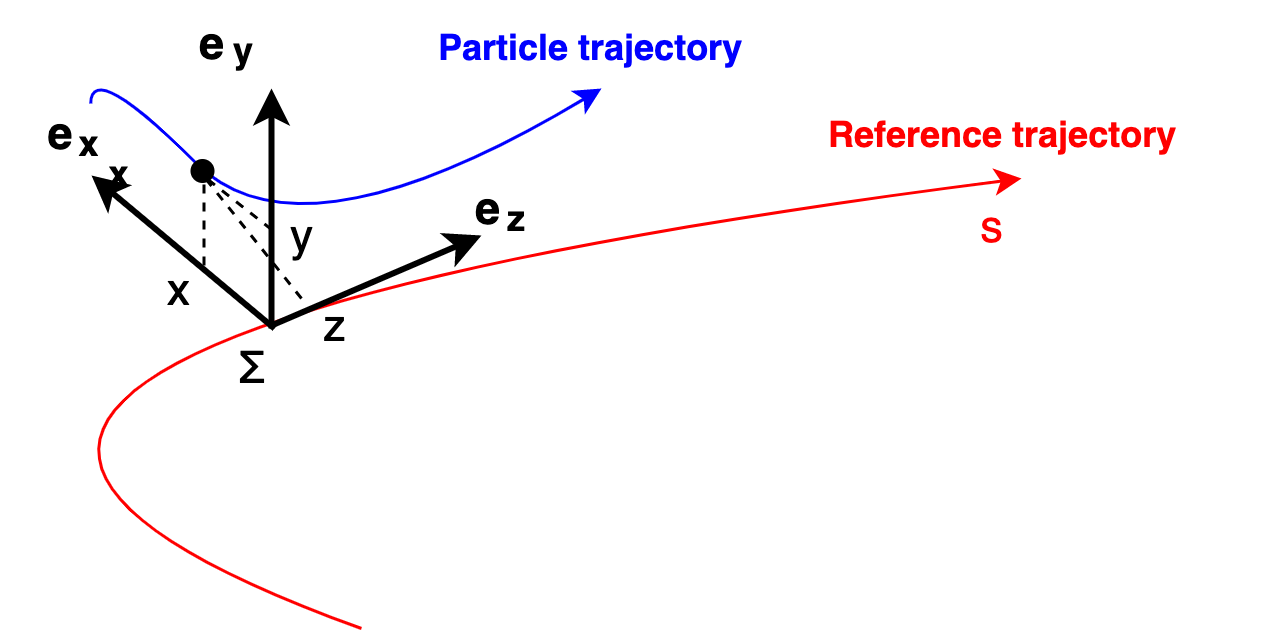
\includegraphics[width=0.8\textwidth]{images/Ch2/coordinates_particle_motion.png}
        \caption{Co-ordinate system used to describe particles motion in a synchrotron. This is a rotating co-ordiante system, with $(\mathbf{e_x, e_y, e_z})$ being the unit vectors, which follows the reference trajectory along the accelerator.}
        \label{fig:coordinate_system}
 \end{figure}


 At any point $s$ along the reference trajectory each particle is represented by the following 6-dimensional vector $(x, x^{\prime}, y, y^{\prime}, z, \delta)$ where:

 \begin{subequations}\label{eq:particle_coordinates}
    \begin{equation}
        x^\prime = \frac{dx}{ds} = \frac{dx}{dt}\frac{dt}{ds} = \frac{v_x}{v_z} =  \frac{p_x}{p_z} \approx \frac{p_x}{p_0},
    \end{equation}    
    \begin{equation}
        y^\prime = \frac{dy}{ds} = \frac{dy}{dt}\frac{dt}{ds} = \frac{v_y}{v_z} =  \frac{p_y}{p_z} 	\approx \frac{p_y}{p_0},
    \end{equation} 
    \begin{equation}
        \delta = \frac{\Delta p}{p_0} = \frac{p-p_0}{p_0},
    \end{equation}
\end{subequations}

where $p_0$ is the momentum of the reference particle as defined in the previous paragraph.
%is the momentum of the reference particle which is given by: $p_0 = \gammarel m_0 v_0$, where $m_0$ is the proton rest mass and

It can be seen that $x^\prime$ and $y^\prime$ are basically the normalised momenta with the reference momentum $p_0$ and $\delta$ is the relative momentum offset from the reference particle. The co-ordinates and the momentum of the reference particle are ($x=y=z=0$) and ($p_x=p_y=0, p_z=p_0$) respectively.

Furthermore, if the direction of motion of the particle has a small angle with the reference trajectory, the paraxial approximation is valid: $p_x, p_y \ll p_z = p_0$ which means that $x^\prime \approx p_x$ and  $y^\prime \approx p_y$. This approximation is valis for the studies presented in this thesis. \textcolor{red}{$p_0=1$? not clear to me} % ultra relativistic regime, is not mentioned at wolski's book. I wrote it for the p_ 0= 1. but i am not sure.
% p.149 wolski and p.12 Michael schenk

%Initial I have written: Furthermore, the ultra-relativistic regime, the transverse momentum/velocity of a particle is very small comparing to the longitudinal one. Therefore the paraxial approximation is used: $p_x, p_y \ll p_z = p_0 = 1$ which can be applied to simplify Eqs.~\ref{eq:particle_coordinates}. %Or see Andy's explanation for low emittance storage rings: https://cds.cern.ch/record/1982424/plots

To summarize, the motion of the particles is separated in the transverse and longitudinal planes where it is described with the  $(x, x^\prime, y, y^\prime)$ and $(z, \delta)$ co-ordinates respectively. In order to avoid a possible misconception it seems appropriate to clarify here, that the longitudinal parameter $z$ indicates the longitudinal offset from the reference particle at the center of the bunch. If $z>0$ ($z < 0$) the corresponding particle reaches earlier (later) than the center of the bunch at an arbitrary reference point.


%\textbf{Further comments}
%\begin{itemize}[noitemsep, topsep=-8pt]  %topsep to remove the space after the %"Further comments"
%    \item In the ultra-relativistic regime, the transverse momentum/velocity of a particle is very small comparing to the longitudinal one. Therefore the paraxial approximation is used: $p_x, p_y \ll p_z = p_0 = 1$ which can be applied to simplify Eqs.~\ref{eq:particle_coordinates}. %Or see Andy's explanation for low emittance storage rings: https://cds.cern.ch/record/1982424/plots
%    \item 
%\end{itemize}
% z = s-u0*t

\section{Single-particle beam dynamics}
In this first section, the interactions between the particles within a bunch are neglected, hence the term single-particle beam dynamics.

\textbf{Two-dimensional complex fields}\\
As already discussed, the motion of the charged particles inside a circular accelerator is controlled by magnetic fields. In this thesis, the magnets are considered purely transverse elements. Their effect is therefore described with two-dimensional multipole fields, acting in the horizontal and vertical planes\footnote{Examples of three-dimensional treatment can be found in~\cite{wolski2014, Beth:889480}. However, the two-dimensional treatment is most often used in accelerator physics as it provides a good description for the majority of the magnetic elements.}. % Wolski Ch1.3, p.33

The description of two-dimensional magnetic fields in accelerator physics is discussed using the concept of multipole expansion and is expressed as a complex quantity. The complex quantity it allows to describe a two-dimensional field in $(x,y)$ space (to be compatible with the co-ordinates used for describing the particle's trajectory as discussed in the previous section). Therefore, the magnetic field around the beam is expressed as follows~\cite{wolski2014}: 
\begin{equation}\label{eq:mult_expansion} % Andy Eq.1.29 + M Schenk Eq.2.2
    B_y(x,y) + i B_x(x,y) = \sum_{n=1}^{\infty} C_n (x+i y)^{n-1},
\end{equation} % principle of superposition 
where $n$ indicates the order of the field component: $n$=1 for a dipole (steering), $n$=2 for quadrupole (focusing (chromticity correction), $n$=4 for octupole (error or field correction) etc. $C_n=(b_n +i \alpha_n)$ is a complex constant which denotes the strength and orientation of the multipole field. The coefficients $b_n=\frac{1}{(n-1)!} \frac{\partial^{n-1}B_y}{\partial x^{n-1}}$ and $\alpha_n=\frac{1}{(n-1)!} \frac{\partial^{n-1}B_x}{\partial x^{n-1}}$ denote the strength of a normal and skew (normal multipole rotated by $\pi/2(n-1)$) multipole respectively in units of $\mathrm{T/m^{n-1}}$.
% Equations for coefficients, sofia's thesis Eq.(2.29) p. 23: https://cds.cern.ch/record/2743602/files/CERN-THESIS-2020-169.pdf

Usually, in accelerator physics the values of the multipole strengths are quoted normalised to the magnetic rigidity as defined in Eq.~\eqref{eq:Brho} and are denoted by:
\begin{equation}\label{eq:kn}
    k_n = \frac{b_n}{B_0 \rho},
\end{equation}
and is expressed in untis of  $\mathrm{T/m^{n}}$. This is the convention that will be used in this thesis.

\subsection{Transvserse motion}
In the transverse plane the motion is orthogonal to the reference trajectory (see Fig.~\ref{fig:coordinate_system}) and its co-ordinates are $(x, x^\prime, y, y^\prime)$. For the discussion on the transverse beam dynamics, the $(x, x^\prime)$ and $(y, y^\prime)$ co-ordinates will be both described by $(u, u^\prime)$ when possible to facilitate the notation.

\textbf{Linear dynamics}\\
Here the transverse motion of a particle moving the two-dimensional fields described in Eq.~\eqref{eq:mult_expansion} is discussed. For now the discussion is limited only in dipolar and quadrupolar components ($n=1$ and $n=2$) hence the name linear dynamics.

As mentioned above, the particles (but the reference one) transversely  oscillate around the reference trajectory. This motion, through an arbitrary periodic sequence of dipoles and quadrupoles is called betatron motion and can be described with the following equations of motion~\cite{Lee:1425444}:
% also sofia's thesis Eq.(2.37)

\begin{equation}\label{eq:transverse_eq_x}
    x^{\prime \prime} - \frac{\rho+x}{\rho^2} = - \frac{B_y}{B_0 \rho} \frac{p_0}{p} \left (  1+ \frac{x}{\rho} \right )^2, 
\end{equation}

\begin{equation}\label{eq:transverse_eq_y}
    y^{\prime \prime} = \frac{B_y}{B_0 \rho} \frac{p_0}{p}  \left (  1+ \frac{x}{\rho} \right )^2, 
\end{equation}

where $s$ is the distance along the reference trajectory, $B_0 \rho$ and $\rho$ the magnetic rigidity and radius as defined in Eq.~\eqref{eq:Brho},  $B_y, B_x$ the transverse magnetic fields of Eq.~\eqref{eq:mult_expansion}, and $p_0$ the reference momentum.

For on-momentum particles ($\delta = 0$) the above betatron equations of motion are simplified to the equation of harmonic oscillator, named the Hill's equation:

\begin{equation}\label{eq:Hills_equation_1}
    u^{\prime \prime}(s) + K_u(s) u(s) = 0,
\end{equation}

where $u=(x,y)$ and:

 \begin{equation}\label{eq:Hills_equation_2}
    K_u(s) = \begin{dcases}
        \frac{1}{\rho(s)}+k(s), & u=x \\
        -k(s), & u=y 
    \end{dcases}
\end{equation}

It should be noted that for Eq.~\eqref{eq:Hills_equation_1} it is assumed that the motion in horizontal and vertical plane are independent (un-coupled).

\textbf{Matrix formalism}\\
The solutions of the Hill's equation can be expressed using matrix formalism as: 
\begin{equation}\label{eq:matrix_formalism_intro}
   \begin{pmatrix}
    u\\ 
    u^\prime
    \end{pmatrix}_{s} = M_u (s |  s_0) \begin{pmatrix}
    u\\ 
    u^\prime
    \end{pmatrix}_{s_0},
\end{equation}

where $u=(x,y)$ and $M$ is the transfer matrix from the position $s_0$ to the $s$.

\textbf{Non-linear dynamics}\\


\subsection{Longitudinal motion}
In the longitudinal plane the motion is tangential to the reference trajectory and is described by the co-ordinates $(z, \delta)$. 


\section{Collective effects}
\subsection{Beam transverse impedance}

\section{Optics models of accelerators}
% or optics design
\subsection*{MADX}
Table with parameters for sps lattice, eg average beta function, tune etc. circumference, Q20 and Q26.

presentation AUTH?


See sondre's thesis for inspiration on the structure.
\section{General parameters of the studies}
% Maybe this should be mentioned at the end of project objectives and thesis outline.
% The following paragraphs are taken from the APR Ch.1.3 
\subsection{SPS optics}\label{subsec:SPS_optics_model}
 The studies presented in this thesis were performed for the nominal SPS optics for the LHC filling which are called Q26 optics as the higher integer part of the tune in both planes is 26. 

 \normalsize{\textbf{SPS nominal model}\\
 The model for the Q26 optics can be found in the official CERN repository~\cite{SPS_optics_repo} and will be referred to as the nominal SPS model in this thesis. The values of the optics parameters in what follows correspond to the model values unless stated otherwise.

 \normalsize{\textbf{SPS non-linear model}\\
\textcolor{red}{Move this section to chapter 6.}
The nominal SPS model includes only the nonlinear fields produced by the chromatic sextupoles. However, one of the most important sources of non-linearities in SPS are the odd multipole components of its main dipole magnets. For some of the studies presented in this thesis their impact on the beam dynamics must be studied and therefore they should be included in the nominal model. 

% APR Chapter 3.1
The multipole error of the SPS main dipoles are unfortunately not available from magnetic measurements. On this ground a non-linear optics model of the SPS has been established with beam-based measurements of the chromatic detuning over a range of momentum deviation~\cite{Carlà:2664976, Alekou:2640326}.  The optics model was obtained by assigning systematic multipole components to the main lattice magnets, in the nominal model of SPS, in order to reproduce the tune variation with themomentum deviation as it was measured in the real machine. The calculations were performed with MAD-X [].

The values of the multipole components up to seventh order obtained from this method are given in Table~\ref{tab:sps_mult_270GeV} where, ($b_3^A, b_3^B$) ($b_5^A, b_5^B$) and ($b_7^A, b_7^B$) stand for the sextupolar, decapolar and decatetrapolar mutipoles respectively. Note that different values have been obtained foreach of the two different kinds of SPS main dipoles (MBA and MBB) which are marked withthe indices A and B respectively.

\begin{table}[ht] % table take from the APR
    \caption{Multipole errors from SPS non-linear model, at 270\,GeV.} % title of Table
    \centering % used for centering table
    \begin{tabular}{c c c c} % centered columns (4 columns)
    \hline\hline %inserts double horizontal lines
    Multipole & Value  \\ [0.5ex] % inserts table
    %heading
    \hline  % inserts single horizontal line
    $b_3^A, b_3^B$ & 8.1 $\times 10^{-4}$\,$\mathrm{m^{-2}}$, 1.1 $\times 10^{-3}$\,$\mathrm{m^{-2}}$\\ 
    $b_5^A, b_5^B$ & 9.2\,$\mathrm{m^{-4}}$, $-$10\,$\mathrm{m^{-4}}$ \\
    $b_7^A, b_7^B$ & 1.3 $\times 10^{5}$\,$\mathrm{m^{-6}}$, 1.4 $\times 10^{5}$\,$\mathrm{m^{-6}}$\\ [1ex] % [1ex] adds vertical space
    \hline %inserts single line
    \end{tabular}
    \label{tab:sps_mult_270GeV} % is used to refer this table in the text
    \end{table}


\textbf{random multiple errros? } Like in APR.Ch.3.2.2.

\section{Luminosity}


    $\mathcal{L} = \frac{n_b f_\mathrm{rev}N_1 N_2}{4 \pi \sigma_x \sigma_y} \frac{1}{\sqrt{1+(\frac{\sigma_z}{\sigma_\mathrm{xing}} \frac{\alpha}{2})^2}} $


% From: https://indico.cern.ch/event/634251/contributions/2566349/attachments/1447935/2231509/impact-crossing-angle.pdf
\section{Emittance}

\textbf{Defintion 1}: The statistical emittance is expressed in terms of the beam distribution: % Wolski Eq. (4.101)

\begin{equation}\label{eq:statistical_definition_emit}
    \epsilon_x^{\mathrm{geom}} = \sqrt{\langle x^2 \rangle - \langle px^2 \rangle - \langle x px \rangle^2}.
\end{equation}
This is the geometric emittance. 
\begin{equation}\label{eq:emit_geom_norm_relation}
    \epsilon_x = \epsilon_x^{\mathrm{geom}} \betarel \gammarel.
\end{equation}


\textbf{Defintion 2}:
For a gaussian beam distribution the normalised beam emittance it applies:
\begin{equation}\label{eq:emit_from_beam_size}
    \epsilon_{x} = \frac{\sigma_x(s)^2 - \delta^2 D_x^2(s)}{\beta_x(s)} \betarel \gammarel
\end{equation}

where $\sigma_x(s)$ is the beam size, $\beta_x(s)$ is the beta function, $D_x(s)$ is the dispersion fat a specific location s along the accelerator, $\delta=\Delta p/p0$ is the momentum spread and $\betarel, \gammarel$ the relativistic parameters. Similar expression is valid for the vertical plane, with the difference that there is no dispersion.

\section{Transfer maps}
Need to mention them briefly as you refer to them at the PyHEADTAIL section.

% Courant snyder formalism of longitudinal dynamics: https://journals.aps.org/prab/pdf/10.1103/PhysRevAccelBeams.24.094001
\section{Action angle variables}
The action for the x-plane is:

\begin{equation}\label{eq:action}
    \Jx = \frac{1}{2}(x_n^2 +xp^2_n) 
\end{equation}
where 
\begin{equation}\label{normalised_y}
    x_n = \frac{x}{\sqrt{\beta_x}}, \ \ xp_n = \frac{\alpha_x x}{\sqrt{\beta_x}} + \sqrt{\beta_x}xp
\end{equation}
the normalised coordinates and $\alpha_y, \beta_y$ the twiss parameters. 
The same applies for the y-plane. 

s
The statistical geometric emittance equals the average of the actions distribution:
\begin{equation}\label{eq:geom_emit_actions}
    \emitxgeom = \langle \Jx \rangle
\end{equation}
%\begin{equation}\label{eq:geom_emit_actions}
%    \epsilon_x^{\mathrm{geom}} = \langle \Jx \rangle
%\end{equation}
The distribution of actions is an exponential distribution (further explanation needed?). Therefore, its mean equals its standard deviation. (this property is used in the appendix for the computation of the rms tune spread.)

From Eq.~\eqref{eq:action} we write:
\begin{equation}\label{eq:Jy_exp_distr}
    e^{-J/\epsilon} = e^{(-x^2/2\epsilon - px^2/2\epsilon)}
\end{equation}
From this equation it can be seen that the actions follow an exponential distribution. 

\section{Wakefields and impedances}\label{sec:wakefields_theory}

he terms dipolar and quadrupolar have been chosen as the dipolar wake function acts on the test proton like a dipole magnet (the kick is the same whatever its transverse location), whereas the quadrupolar term acts like a quadrupole magnet (the kick increases linearly with the transverse offset of the test particle). Benoits thesis p.44


\section{Tracking simulation codes}\label{sec:simualtion_codes}
In this section the two tracking simulation codes used in this thesis to study the noise-induced emittance growth are presented. Both codes are macroparticle tracking libraries that simulate the particle motion in the six-dimensional (6D) phase space $(x, x^\prime, y, y^\prime, z, \delta)$. The first code performs tracking between interaction points around a circular accelerator with the use of trasnfer matrices while the second one uses the detailed optics model of the machine.

\subsection{PyHEADTAIL}\label{subsec:pyheadtail}

PyHEADTAIL~\cite{pyheadtail_repository} is an open-source 6D macroparticle tracking code, developed at CERN, which was originally designed to study collective effects in circular machines and to be easily extrensible with custom elements. 
% https://indico.cern.ch/event/930271/contributions/3910265/attachments/2066139/3467770/30June2020_Simulations_emit_growthCC_RFnoise.pdf  
Details on its implementation and its features can be find in Refs.~\cite{pyheadtail_manual_adrian, pyheadtail_schenk}. Below the main steps of a simulation are listed: % according to the interest of this thesis.

% Thesis david: https://cds.cern.ch/record/2707064/files/CERN-THESIS-2019-272.pdf (p.45) and for the transverse matrix.

\begin{enumerate}
    \item \textbf{Machine initialisation:} The accelerator ring is splitted into a number of segments of equal length, after each of which there is an interaction point (IP). At the interaction points the macroparticles experience kicks from various accelerator components (feedback system, multipoles etc) or from collective effects such as the wakefields. The machine parameters, such as the circumference, the betatron and synchrotron tunes and the optics at the interaction points are defined. It should be noted that PyHEADTAIL uses smooth approximation which means that only a few segments are defined per turn. % which results to a very  rough optics model.
    \item \textbf{Bunch initialisation:}  A particle bunch is represented by a collection of macroparticles, each of which represents a clustered collection of physical particles. Each macroparticle is described by four transverse $(x, x^\prime, y, y^\prime)$ and two longitudinal coordinates $(z, \delta)$, a mass and an electric charge. For the studies presented in this thesis $10^{5}$ macroparticles are sufficient for an accurate represantation of the bunch, unless it is stated otherwise. There are various distributions available. In this thesis the simulations are performed using a Gaussian distribution in transverse and longitudinal planes.
    \item \textbf{Transverse tracking}: In the transverse plane, the macroparticles are transported from one interaction point to another by linear transfer matrices which take into account the optics parameters at the beginning and the end of the corresponding segment. For example, in the horizontal plane the transport of each macroparticle from IP1 to IP2 along the ring is given by:
    \begin{equation}
        \binom{x_i}{x_i^\prime}_{\mathrm{IP0}} = M \binom{x_i}{x_i^\prime}_{\mathrm{IP1}},
    \end{equation}
    where $i=1, ..., N$ with N being the number of macroparticles and the matrix $M$ is given by:
    \begin{equation}\label{eq:linear_transfer_map}
        M = \begin{pmatrix}
            \sqrt{\beta_{x, \mathrm{IP0}}} & 0 \\ 
            -\frac{\alpha_{x, \mathrm{IP0}}}{\sqrt{\beta_{x,  \mathrm{IP0} }}} & \frac{1}{\sqrt{\beta_{x, \mathrm{IP0}}}}
            \end{pmatrix} \begin{pmatrix}
                \cos(\Delta \mu_{x, \mathrm{IP0 \to IP1 }}) & \sin(\Delta \mu_{x, \mathrm{IP0 \to IP1 }})\\
                 - \sin(\Delta \mu_{x, \mathrm{IP0 \to IP1 }})  &\cos(\Delta \mu_{x, \mathrm{IP0 \to IP1 } }) 
                \end{pmatrix}  \begin{pmatrix}
                    \sqrt{\beta_{x, IP1}} & 0 \\ 
                    -\frac{\alpha_{x, IP1}}{\sqrt{\beta_{x, IP1}}} & \frac{1}{\sqrt{\beta_{x, IP1}}}
                    \end{pmatrix} 
    \end{equation}
    where $\alpha_{x, \mathrm{IP0/IP1}}$ and $\beta{x, \mathrm{IP0/IP1}}$ are the optics paramters at the interaction points IP0 and IP1 respectively and $\Delta \mu_{x, \mathrm{IP0 \to IP1 }}$ the phase advance from IP0 to IP1. As smooth approximation is used, the phase advance equals: 
    \begin{equation}\label{eq:phase_advance_smooth_approximation}
        \Delta \mu_{x, \mathrm{IP0 \to IP1 }} = Q_x \frac{L}{C},
    \end{equation}
    where $Q_x$ is the horizontal betatron tune, $C$ the machine circumference and $L$ the length of the corresponding segment. It should be noted that if no detuning source is added (see next step) the matrix $M$ is the same for all particles.
    \item \textbf{Chromaticity and detuning with transverse amplitude:} The chromaticity (up to higher orders) and amplitude detuning are implemented as a change of the phase advance of each individual particle as follows (example for the horizontal plane):
    \begin{equation}\label{eq:change_phase_advance_detunign}
        \Delta \mu_{x, i \mathrm{IP0 \to IP1 }} = \Delta \mu_{x, \mathrm{IP0 \to IP1 }} + (\xi^{1}_x \delta_i + \alpha_{xx}J_{x, i} + \alpha_{xy}J_{y,i}) \frac{\Delta \mu_{x, \mathrm{IP0 \to IP1 }}}{2\pi Q_x}, 
    \end{equation}
    where $i=1, ..., N$ with N being the number of macroparticles, $\Delta \mu_{x, \mathrm{IP0 \to IP1 }}$ is the phase advance for all macroparticles defined in the previous step, $\xi_x^{1}$ the horizontal chromaticity of first order normalised to the tune $\alpha_{xx}$ and $\alpha_{xy}$ are the detuning coefficients, while $J_x$ and $J_y$ are the horizontal and vertical actions of the macroparticle. Therefore, in the presence of detuning the elements of the $M$ matrix are different for every particle.

    \item \textbf{Longitudinal tracking:}  In PyHEADTAIL the longitudinal particle dynamics are described with the longitudinal equations of motion (ref to eq earlier.) % slide 37: https://www2.kek.jp/accl/legacy/seminar/file/PyHEADTAIL_PyECLOUD_2.pdf 
    The longitudinal coordinates are advanced once per turn after solving numerically the equations of motion~\cite{pyheadtail_schenk}. The motion can be linear or not (non-linear RF system). The studies presented in this thesis use the linear longitudinal tracking.

    \item \textbf{Trasnverse impedance effects:} In PyHEADTAIL, wakefield kicks are used to implement the effect of the transverse impedance in time domain. To improve the computational efficiency, the total impedance of the full machine is lumped in one of the interaction points along the ring and the kicks are applied on the macroparticles once per turn. Additionally, instead of computing the wakefield kicks from each particle to the rest individually, the bunch is divided in a number of longitudinal slices and the macroparticles in each slice recieve a wakefield kick generated by the preceding slices\footnote{This is valid in the ultrarelativistic scenario when no wakefield is generated in front of the bunch. The condition applies for the SPS experiments described in this thesis, performed at 270\,GeV.}~\cite{Salvant:1274254}. This is illustrated schematically in Fig.~\ref{fig:longitudinal_slicing_wakefields}. A large number of slices is required such as the wakes can be assuemed constant within the slice. A high number of macroparticles is also needed in order to avoid statistical noise effects caused by undersampling~\cite{pyheadtail_manual_adrian}. For the studies presented in 500 slices are used over a range of three rms bunch lengths in both directions from the bunch center with the bunch being represented by $10^6$ macroparticles (instead of $10^5$ required for simulations without impedance effects).
    

    \begin{figure}[!ht]
        \centering
        \begin{subfigure}[t]{0.45\textwidth}
            \centering
            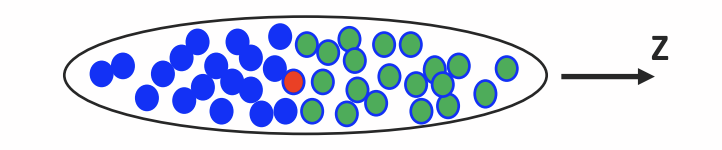
\includegraphics[width=1\textwidth]{images/Ch2/before_slicing.png}
            \caption{Without slicing}
            %\label{fig:add_label_here}
        \end{subfigure}
        \hfill
        \begin{subfigure}[t]{0.45\textwidth}
            \centering
            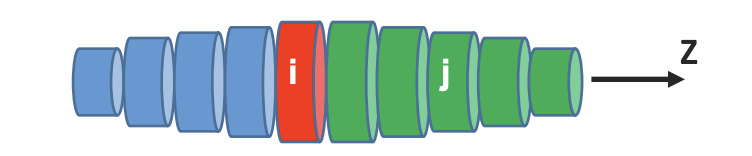
\includegraphics[width=1\textwidth]{images/Ch2/after_slicing.png}
            \caption{With slicing}
            %\label{fig:add_label_here}
        \end{subfigure}
        \hfill
         \caption{Longitudinal bunch slicing for the implementation of wakefields kicks in PyHEADTAIL. Without the slicing technique (left) the wake kicks on the red macroparticle are generated from all the green macroparticles resulting to computationally heavy simulations. Instead, when the bunch is sliced longitudinally (right) the wake kicks on the macroparticles in the red slice $i$ are generated by the macroparticles in the green slices $j$, decreasing significantly the computation time. The figures are a courtesy of M. Schenk~\cite{pyheadtail_schenk}} % bunch passage
         \label{fig:longitudinal_slicing_wakefields}
     \end{figure}
        
    The wakefield kicks are computed using a convolution of the wake function with the moments of each particle. %p.39 michael schenk thesis
    The wake functions are available from detailed imepdance model of the machine which are obtained from a combination of theoretical computations, electromagentic simulations and can be imported in PyHEADTAIL in form of tables. More details on the SPS impedance model are provided in Section~\ref{sec:sps_impedance_model}.
    
    \item \textbf{Data acquisition:} The updated bunch coordinates after each turn are available at IP0 for post processing. Typically, $10^{5}$ turns are required for the noise-induced emittance growth simulation presented in this thesis. 
    
\end{enumerate}


%Last sentence from (LinearMap): https://github.com/PyCOMPLETE/PyHEADTAIL/blob/master/PyHEADTAIL/trackers/longitudinal_tracking.py
%or longutidanl equations of motion: slide 37 https://www2.kek.jp/accl/legacy/seminar/file/PyHEADTAIL_PyECLOUD_2.pdf

Figure~\ref{fig:pyheadtail_accelerator_model} shows a graphic representation of the accelerator model and the tracking procedure supporting the steps described above.
% Graph is created app.diagrams.net and is saved in goodle dirve.

\begin{figure}[!h]
    \centering         
    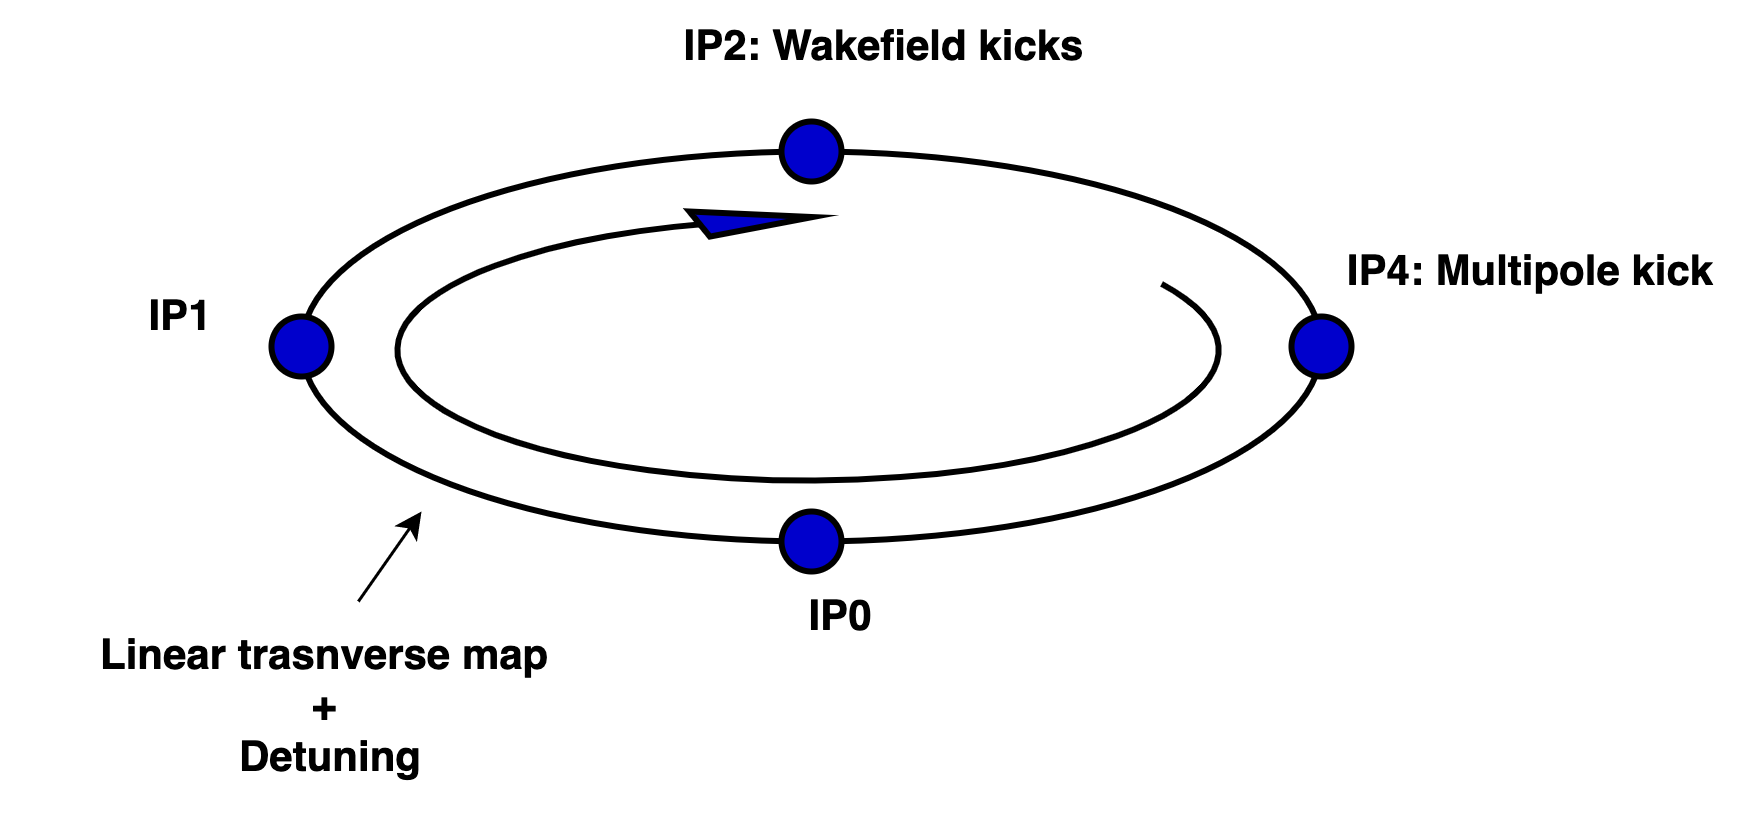
\includegraphics[width=0.6\textwidth]{images/Ch2/accelerator_model_graph_pyheadtail.png}
        \caption{Graphic represantation of the accelerator model and tracking procedure in PyHEADTAIL (inspered by the graphs in Refs.~\cite{pyheadtail_schenk, inproceedings_ibs_pyheadtail}). In this example the ring is splitted in four segments seperated by the interaction points (IPs). Wakefield and mulitple kicks are applied on the macroparticles in IP2 and IP4. The macroparticles are transported between the IPs by a linear map (which can include detuning effects) in the transverse plane.  The longitudinal coordinates are updated once per turn without being visualised in this plot.}
        \label{fig:pyheadtail_accelerator_model}
 \end{figure}


\subsection{Sixtracklib}\label{subsec:sixtracklib}
%Introduction to sixtrackib: https://indico.cern.ch/event/833895/contributions/3577803/attachments/1927226/3190636/intro_sixtracklib.pdf
% https://inspirehep.net/files/6273430c727ace3796a92d069f651ade